\documentclass[12pt]{beamer}

\mode<presentation> {
	
	
	%\usetheme{Madrid}
	%\usepackage{times}
	\renewcommand{\familydefault}{\rmdefault}
	\usetheme{CambridgeUS}
	\usepackage[latin1]{inputenc}
	\usefonttheme{professionalfonts}
	\usepackage{times}
	\usepackage{tikz}
	\usepackage{amsmath}
	\usepackage{verbatim}
    \usepackage{graphicx}
	\usepackage{enumerate}
	\usepackage{setspace}
	\usetikzlibrary{arrows,shapes}
	\usepackage{amsmath}
	\usepackage{eurosym}
	\usepackage{framed}
	\usepackage{extarrows}
}

\usepackage{graphicx}
\usepackage{booktabs}
\usepackage{url}

%----------------------------------------------------------------------------------------
%	TITLE PAGE
%----------------------------------------------------------------------------------------


\title{VaR on CMS Stock}

\author[$Group 13$]{Presenter:\ \  Group 13 }
\institute[]{
	\textsl{By: Huang Junfeng, Wu Peikun, Sun Liang, Cao Chunyu}
}
\date[July 10$\ {th}, 2016$]{}


\begin{document}
	
\begin{frame}
	\titlepage
\end{frame}


\begin{frame}
	\frametitle{Outline}
	\tableofcontents
\end{frame}

\section{Definition of VaR}
\begin{frame}
	\frametitle{Definition of VaR}
	\begin{itemize}
		\item Value at Risk (VaR) is a measure of the risk of investments. It estimates how much a set of investments might lose, given normal market conditions, in a set time period such as a day. VaR is typically used by firms and regulators in the financial industry to gauge the amount of assets needed to cover possible losses.
		\item VaR is defined as: for a given portfolio, time horizon, and probability p, the p VaR is defined as a threshold loss value, such that the probability that the loss on the portfolio over the given time horizon exceeds this value is $p$. This assumes mark-to-market pricing, and no trading in the portfolio.
		
		\item Mathematical definition:
\\$VaR_\alpha(L)$$=inf\{l\in\Re:P(L>l)\leqslant1-\alpha\}$\\$\ \ \ \ \ \ \ \ \ \ \ \ \ \ \ \ =inf\{l\in\Re:F_L(l)\geqslant\alpha\}$

	\end{itemize}
\end{frame}


\section{Our Project}
\begin{frame}
	\frametitle{Our Project}
	\begin{itemize}
		\item Apply Value at Risk Technics Using Delta Normal Method to  Share of China Merchants Securities Co. Ltd.(CMS) Listed in the Shanghai Securities Exchange,China(Trading code: 600999).
        \item Used Algorithm:   \\VaR by Delta Normal Method with RMA and EMA.
        \item Selected Data: \\Daily Closing Price of CMS from January 4,2010 to July 8,2016.
\item Output:   \\ VaR Analysis Results by RMA and EMA Estimating Methods Respectively.
	\end{itemize}
\end{frame}


\section{The Result}
\begin{frame}
	\frametitle{\textbf{The Result}}
	\begin{itemize}

		\item VaR on CMS Stock
	\end{itemize}
\begin{figure}
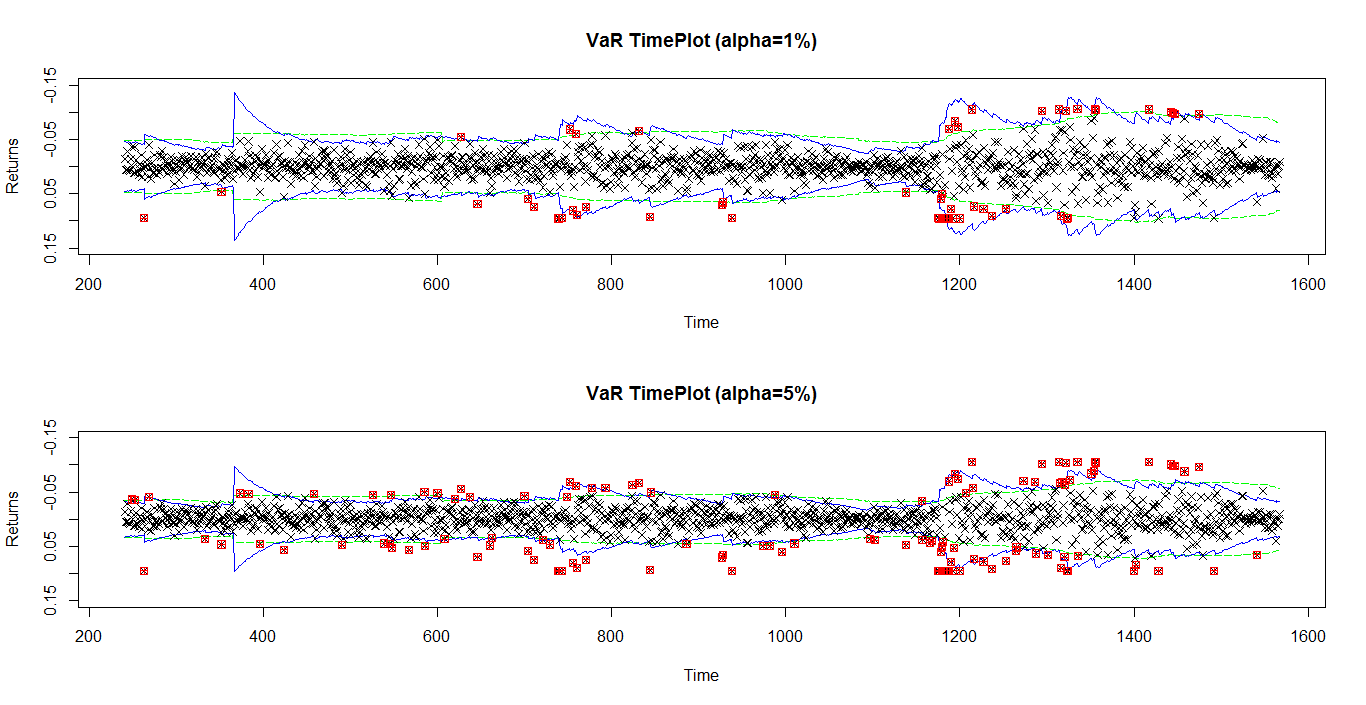
\includegraphics[scale=0.27]{VaRtoCMSStock.png}
\caption{Observed changes of the portfolio values (dots) Lt . Predicted
VaRs based on RMA (dashed line) and EMA (solid line) at $5\%$ and $1\%$}
    \end{figure}
\end{frame}


\section{Project Items}
	\begin{frame}
		\frametitle{Project Items}
\begin{itemize}
		\item The original data is saved as $CMS.txt$ which includes Daily Closing Price of CMS Stock from January 4,2010 to July 8,2016.
\
        \item The code of R is save as $VaRtoCMSStock.R$ for functional implementation of VaRs based on RMA and EMA.
            \
        \item The result is plotted as the png file $VaRtoCMSStock.png$ as to show the predicted
VaRs based on RMA and EMA.\
        \item The meta information is save as $metainfo.txt$ following the instructions from \textbf{Styleguide-and-FAQ}.

	\end{itemize}
\end{frame}
	\begin{frame}
		\frametitle{ }
		\Huge{\centerline{Thank You!}}

	\end{frame}
	
	%----------------------------------------------------------------------------------------
	
\end{document}
